\documentclass[man,floatsintext]{apa6}
\usepackage{lmodern}
\usepackage{amssymb,amsmath}
\usepackage{ifxetex,ifluatex}
\usepackage{fixltx2e} % provides \textsubscript
\ifnum 0\ifxetex 1\fi\ifluatex 1\fi=0 % if pdftex
  \usepackage[T1]{fontenc}
  \usepackage[utf8]{inputenc}
\else % if luatex or xelatex
  \ifxetex
    \usepackage{mathspec}
  \else
    \usepackage{fontspec}
  \fi
  \defaultfontfeatures{Ligatures=TeX,Scale=MatchLowercase}
\fi
% use upquote if available, for straight quotes in verbatim environments
\IfFileExists{upquote.sty}{\usepackage{upquote}}{}
% use microtype if available
\IfFileExists{microtype.sty}{%
\usepackage{microtype}
\UseMicrotypeSet[protrusion]{basicmath} % disable protrusion for tt fonts
}{}
\usepackage{hyperref}
\hypersetup{unicode=true,
            pdftitle={Tutorial of moderated mediation with SEM: the gemm package},
            pdfauthor={Peter Verboon~\& Gjalt-Jorn Peters},
            pdfkeywords={moderated mediation SEM Lavaan},
            pdfborder={0 0 0},
            breaklinks=true}
\urlstyle{same}  % don't use monospace font for urls
\usepackage{color}
\usepackage{fancyvrb}
\newcommand{\VerbBar}{|}
\newcommand{\VERB}{\Verb[commandchars=\\\{\}]}
\DefineVerbatimEnvironment{Highlighting}{Verbatim}{commandchars=\\\{\}}
% Add ',fontsize=\small' for more characters per line
\usepackage{framed}
\definecolor{shadecolor}{RGB}{248,248,248}
\newenvironment{Shaded}{\begin{snugshade}}{\end{snugshade}}
\newcommand{\KeywordTok}[1]{\textcolor[rgb]{0.13,0.29,0.53}{\textbf{#1}}}
\newcommand{\DataTypeTok}[1]{\textcolor[rgb]{0.13,0.29,0.53}{#1}}
\newcommand{\DecValTok}[1]{\textcolor[rgb]{0.00,0.00,0.81}{#1}}
\newcommand{\BaseNTok}[1]{\textcolor[rgb]{0.00,0.00,0.81}{#1}}
\newcommand{\FloatTok}[1]{\textcolor[rgb]{0.00,0.00,0.81}{#1}}
\newcommand{\ConstantTok}[1]{\textcolor[rgb]{0.00,0.00,0.00}{#1}}
\newcommand{\CharTok}[1]{\textcolor[rgb]{0.31,0.60,0.02}{#1}}
\newcommand{\SpecialCharTok}[1]{\textcolor[rgb]{0.00,0.00,0.00}{#1}}
\newcommand{\StringTok}[1]{\textcolor[rgb]{0.31,0.60,0.02}{#1}}
\newcommand{\VerbatimStringTok}[1]{\textcolor[rgb]{0.31,0.60,0.02}{#1}}
\newcommand{\SpecialStringTok}[1]{\textcolor[rgb]{0.31,0.60,0.02}{#1}}
\newcommand{\ImportTok}[1]{#1}
\newcommand{\CommentTok}[1]{\textcolor[rgb]{0.56,0.35,0.01}{\textit{#1}}}
\newcommand{\DocumentationTok}[1]{\textcolor[rgb]{0.56,0.35,0.01}{\textbf{\textit{#1}}}}
\newcommand{\AnnotationTok}[1]{\textcolor[rgb]{0.56,0.35,0.01}{\textbf{\textit{#1}}}}
\newcommand{\CommentVarTok}[1]{\textcolor[rgb]{0.56,0.35,0.01}{\textbf{\textit{#1}}}}
\newcommand{\OtherTok}[1]{\textcolor[rgb]{0.56,0.35,0.01}{#1}}
\newcommand{\FunctionTok}[1]{\textcolor[rgb]{0.00,0.00,0.00}{#1}}
\newcommand{\VariableTok}[1]{\textcolor[rgb]{0.00,0.00,0.00}{#1}}
\newcommand{\ControlFlowTok}[1]{\textcolor[rgb]{0.13,0.29,0.53}{\textbf{#1}}}
\newcommand{\OperatorTok}[1]{\textcolor[rgb]{0.81,0.36,0.00}{\textbf{#1}}}
\newcommand{\BuiltInTok}[1]{#1}
\newcommand{\ExtensionTok}[1]{#1}
\newcommand{\PreprocessorTok}[1]{\textcolor[rgb]{0.56,0.35,0.01}{\textit{#1}}}
\newcommand{\AttributeTok}[1]{\textcolor[rgb]{0.77,0.63,0.00}{#1}}
\newcommand{\RegionMarkerTok}[1]{#1}
\newcommand{\InformationTok}[1]{\textcolor[rgb]{0.56,0.35,0.01}{\textbf{\textit{#1}}}}
\newcommand{\WarningTok}[1]{\textcolor[rgb]{0.56,0.35,0.01}{\textbf{\textit{#1}}}}
\newcommand{\AlertTok}[1]{\textcolor[rgb]{0.94,0.16,0.16}{#1}}
\newcommand{\ErrorTok}[1]{\textcolor[rgb]{0.64,0.00,0.00}{\textbf{#1}}}
\newcommand{\NormalTok}[1]{#1}
\usepackage{graphicx,grffile}
\makeatletter
\def\maxwidth{\ifdim\Gin@nat@width>\linewidth\linewidth\else\Gin@nat@width\fi}
\def\maxheight{\ifdim\Gin@nat@height>\textheight\textheight\else\Gin@nat@height\fi}
\makeatother
% Scale images if necessary, so that they will not overflow the page
% margins by default, and it is still possible to overwrite the defaults
% using explicit options in \includegraphics[width, height, ...]{}
\setkeys{Gin}{width=\maxwidth,height=\maxheight,keepaspectratio}
\IfFileExists{parskip.sty}{%
\usepackage{parskip}
}{% else
\setlength{\parindent}{0pt}
\setlength{\parskip}{6pt plus 2pt minus 1pt}
}
\setlength{\emergencystretch}{3em}  % prevent overfull lines
\providecommand{\tightlist}{%
  \setlength{\itemsep}{0pt}\setlength{\parskip}{0pt}}
\setcounter{secnumdepth}{0}
% Redefines (sub)paragraphs to behave more like sections
\ifx\paragraph\undefined\else
\let\oldparagraph\paragraph
\renewcommand{\paragraph}[1]{\oldparagraph{#1}\mbox{}}
\fi
\ifx\subparagraph\undefined\else
\let\oldsubparagraph\subparagraph
\renewcommand{\subparagraph}[1]{\oldsubparagraph{#1}\mbox{}}
\fi

%%% Use protect on footnotes to avoid problems with footnotes in titles
\let\rmarkdownfootnote\footnote%
\def\footnote{\protect\rmarkdownfootnote}


  \title{Tutorial of moderated mediation with SEM: the gemm package}
    \author{Peter Verboon\textsuperscript{1}~\& Gjalt-Jorn Peters
\textsuperscript{1 }}
    \date{}
  
\shorttitle{Tutorial gemm}
\affiliation{
\vspace{0.5cm}
\textsuperscript{1} Open University}
\keywords{moderated mediation SEM Lavaan}
\usepackage{csquotes}
\usepackage{upgreek}
\captionsetup{font=singlespacing,justification=justified}

\usepackage{longtable}
\usepackage{lscape}
\usepackage{multirow}
\usepackage{tabularx}
\usepackage[flushleft]{threeparttable}
\usepackage{threeparttablex}

\newenvironment{lltable}{\begin{landscape}\begin{center}\begin{ThreePartTable}}{\end{ThreePartTable}\end{center}\end{landscape}}

\makeatletter
\newcommand\LastLTentrywidth{1em}
\newlength\longtablewidth
\setlength{\longtablewidth}{1in}
\newcommand{\getlongtablewidth}{\begingroup \ifcsname LT@\roman{LT@tables}\endcsname \global\longtablewidth=0pt \renewcommand{\LT@entry}[2]{\global\advance\longtablewidth by ##2\relax\gdef\LastLTentrywidth{##2}}\@nameuse{LT@\roman{LT@tables}} \fi \endgroup}



\authornote{

Correspondence concerning this article should be addressed to Peter
Verboon, P.O.Box 2960, 6401 DL Heerlen. E-mail:
\href{mailto:Peter.Verboon@ou.nl}{\nolinkurl{Peter.Verboon@ou.nl}}}

\abstract{
Moderated mediation analysis assumes that the effect of a predictor on a
dependent variable is mediated by one or more mediators and that the
indirect paths in this mediation are moderated. Moderation can take
place on the effect of the predictor on the mediators, or on the effect
of the mediators on the dependent variable.\\
In this tutorial we will show how the package ``gemm'' can be used to do
a moderated mediation analysis.


}

\usepackage{amsthm}
\newtheorem{theorem}{Theorem}[section]
\newtheorem{lemma}{Lemma}[section]
\theoremstyle{definition}
\newtheorem{definition}{Definition}[section]
\newtheorem{corollary}{Corollary}[section]
\newtheorem{proposition}{Proposition}[section]
\theoremstyle{definition}
\newtheorem{example}{Example}[section]
\theoremstyle{definition}
\newtheorem{exercise}{Exercise}[section]
\theoremstyle{remark}
\newtheorem*{remark}{Remark}
\newtheorem*{solution}{Solution}
\begin{document}
\maketitle

\subsection{Introduction}\label{introduction}

In modeling the relation between a predictor and a dependent variable
there are basically three modeling situations to consider. First, there
are other variables that are correlated with the dependent variable, and
possibly also with the predictor. Adding such variables, which are
usually called covariates, to the regression model may change the
regression coefficient of the predictor, and the standard error for this
estimate. This is discussed in many textbooks about multivariate and
regression analysis. Second, the mechanism explaining the effect between
predictor and dependent can be examined by a mediation analysis. The
mediator is a variable that partly \enquote{explains} the assumed causal
process, which links the predictor to the dependent variable. Third, the
effect of interest depends on another variable, which is called the
moderator. A moderator influences the effect of the predictor on the
dependent, implying that the effect is conditional on the value of the
moderator. When the three modeling situations are combined we obtain a
general model, which is useful in many applied research. This general
model is called the moderated mediation model and is earlier described
in the methodological literature (e.g. Edwards and Lambert (2007); Hayes
(2015); Preacher, Rucker, and Hayes (2007)). In this paper a short
description of the moderated mediation model is given. Next the R
package \enquote{gemm} is discussed, which is developed to analyze this
model in an easy and straightforward way. A moderated mediation model
assumes that the effect of a predictor on a dependent variable is
mediated by one or more mediators and that the indirect paths in this
mediation are moderated. Moderation can take place on the effect of the
predictor on the mediators, or on the effect of the mediators on the
dependent variable. In this tutorial the function \texttt{gemm()} is
described for the analysis of moderated mediation models. The function
is an alternative for the (SPSS or SAS) PROCESS macro developped by
Hayes (Hayes, 2018). The \texttt{gemm} is in the R package
\texttt{gemm}. This package can be installed from Github and then loaded
using the \texttt{library()} function:

\texttt{devtools::install\_github("PeterVerboon/gemm")}

\begin{Shaded}
\begin{Highlighting}[]
\KeywordTok{library}\NormalTok{(gemm)}
\end{Highlighting}
\end{Shaded}

An illustration of the moderated mediation model, for which the function
can be applied, is shown in Figure 1. The figure represents a structural
model, linking the observed variables to each other. We are therefore
using the SEM software to fit the moderated mediation model. To this end
we use the lavaan package (Rosseel, 2012). Figure 1 shows the most
general situation, with several mediators, several covariates for the
mediators and several covariates for the dependent variable. There are
also two moderators in this model, one for the paths from the predictor
to the mediators and one for the paths from the mediators to the
dependent variabele.

\begin{figure}
\centering
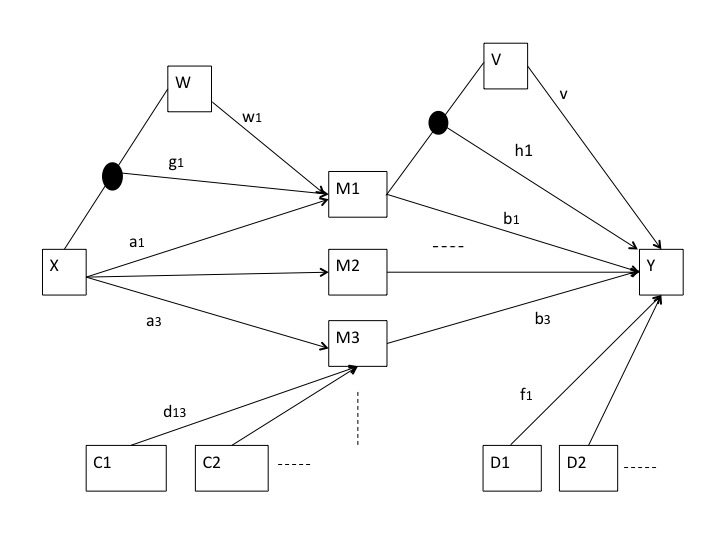
\includegraphics{Figure ModMed model.jpg}
\caption{Moderated mediation model}
\end{figure}

The model is limited in the sense that only one predictor, one dependent
variable, and for each path one moderator are defined. Furthermore,
serial mediation is not included in this model. The number of mediators
and covariates is not limited.

The function \texttt{gemm()} calls the functions
\texttt{buildModMedSemModel()}, which builds the requested SEM model. In
this model we assume that the covariates for the mediators (C) are
correlated with each other, and furthermore that the covariates fir the
dependent variable (D) correlate with each other and also with the
mediators. If covariates (C) are included in the model, paths are
assumed to exist from the covariates (C) to all mediators. For the
function to run the model needs to have a predictor, a dependent
variable and at least one mediator. All other variables are optional.
This most basic model (predictor --\textgreater{} mediator
--\textgreater{} dependent) is just identified: three regression
coefficients are estimated from the covariance matrix, containing three
correlations. With two mediators there are six datapoints, and als six
parameters to estimate (5 regression paths and one covariance between
the mediators). With three mediators there are ten datapoints, and also
ten parameters to estimate (three regression paths and the three
covariances between the mediators). It is easy to see that models with
only mediators, a predictor and a dependent variable, are always just
identified. The fit values for these model s will therefore show perfect
fit. Adding covariates or moderators will result in models in which the
parameters have to be estimated iteratively, yielding model fit values
that indicate how well the model fits the data. After running the
function \texttt{gemm()} there are several functions available that are
designed to handle the results: \texttt{plotSS()}, \texttt{plotIMM()},
\texttt{plotIMM3d()} and \texttt{print()}. These functions will be
illustrated in this tutorial.

\subsection{Index of moderated
mediation}\label{index-of-moderated-mediation}

A primary statistic of interest in moderated mediation models is the
index moderated mediation (Hays, 2015), which can be plotted by
\texttt{gemm}. For a good understanding of this index, we will first
present its algebraic derivation. When there are no moderators or when
moderators take the value zero, the indirect (unmoderated) effect is
defined as: \(a_j b_j\). The indirect moderated effect with the X -- M
path moderated by W (assuming there is no moderation through V or when V
= 0) is derived as follows:

\begin{equation}
 \begin{split}
 M_j = a_j X + w_j W + g_j WX\\
 Y = b_j M_j.
 \end{split}
\end{equation}

Substitute \(M_j\):

\begin{equation}
   \begin{split}
   Y = b_j(a_j X + w_j W + g_j WX)\\
   Y = b_j w_j W + (a_j b_j + b_j g_j W)X.
   \end{split}
  \end{equation}

A quantification the effect of X on Y as a function of the moderator has
been described by Hayes (2015, 2018), who coined the term \enquote{index
of moderated mediation}. The index of moderated mediation (IMM) is
defined here as:

\begin{equation}
  IMM_a = a_j b_j + b_j g_j W.
  \end{equation}

This definition is slightly different from that given by Hayes (2105),
since contrary to Hayes(2015), here it also contains the term constant
term \(a_j b_j\). The IMM for a single path represents the slope (and
intercept) of the line that relates the predictor with the dependent
variable, as a function of the moderator. The index consists of a fixed
part (the indirect effect) and a part that varies with the moderator.
The plot of the IMM versus the moderator can be constructed using
formula (2), which gives a straight line. This plot shows how the
relation between predictor and dependent variable changes when the
moderator changes. A flat horizontal line in this plot indicates that
there is no moderation. A steep line om the other hand indicates a
moderation effect. When W = 0 the IMM represents the indirect
(unmoderated) effect. The single-path IMM is defined for each mediator
separately. Likewise, the IMM is defined for each path separately, thus
for the path from predictor to mediator (a-path) and also for mediator
to the dependent variable (b-path). Foth this reason we refer to it as a
single-path IMM. So, for three mediators and two moderators (one for
each path), six single-path IMMs can be computed. Combining both
moderators to obtain a double-path IMM would give a two-dimensional
plane in a three-dimensional space (instead of a line), defined by the
two moderators and the IMM. The index is derived as follows.

\begin{equation}
 \begin{split}
M_j = a_j X + w_j W + g_j WX\\ 
Y = b_j M_j + vV + h_j M_j V. 
 \end{split}
\end{equation}

Substitute M\_j:

\begin{equation}
 \begin{split}
Y = b_j(a_j X + w_j W + g_j WX) + vV + h_j (a_j X + w_j W + g_j WX)V\\ 
Y = b_j w_j W + (a_j b_j + b_j g_j W)X + vV + h_j w_j WV + (h_j a_j V + h_j g_j WV)X\\ 
Y = b_j w_j W + vV + g_j w_j WV + (a_j b_j + b_j g_j W + h_j a_j V + h_j g_j WV)X. 
 \end{split}
\end{equation}

The two-dimensional IMM, incorporating both moderators is:

\begin{equation}
IMM = a_j b_j + b_j g_j W + h_j a_j V + h_j g_j WV.
\end{equation}

When one of the moderators is dichotomous, it is more convenient to plot
the double-path IMM in a two dimensional space with two lines, one for
each category of the moderator. It is easy to see that formula (6) is a
generalization of formula (3), when V = 0 (or absent), and when W = 0
(or absent), the index of moderated mediation (IMM) of the b-path is
defined as:

\begin{equation}
IMM_b = a_j b_j + h_j a_j V.
\end{equation}

Like before, this index indicates how the slope of the effect of X on Y
changes as a function of the moderator, here the moderator of the b-path
(V)

\subsection{Examples}\label{examples}

The required parameters of the function \texttt{gemm()} can be found by
typing \texttt{?gemm}. This gives the help page of the function. The
fictious data that will be used to illustrate the model are included in
the package and are in the R object \texttt{gemmDat}, which can be
loaded by \texttt{data("gemmDat")}. After loading the data, you can also
learn more about the data by using the question mark.

\begin{Shaded}
\begin{Highlighting}[]
\KeywordTok{data}\NormalTok{(}\StringTok{"gemmDat"}\NormalTok{)          }\CommentTok{# loads the data}
\end{Highlighting}
\end{Shaded}

The data have simple and commonly used variable names: x and y for the
predictor and dependent variable, respectively. The \enquote{m} with a
number represents mediators and the \enquote{c} covariates, numerical
moderators start with \enquote{mod}, and dichotomous moderators with
\enquote{bi}.

\subsection{The mediation model}\label{the-mediation-model}

The first model that will be illustrated is a straightforward mediation
model with three mediators, without moderators and without covariates.
The number of bootstrap samples is set to 100, a very small number for
bootstraps, but here only used for illustration. For a real analysis you
might use 5,000 boostraps; the default for nboot is 1,000.

\begin{Shaded}
\begin{Highlighting}[]
\NormalTok{result <-}\StringTok{ }\KeywordTok{gemm}\NormalTok{(}\DataTypeTok{dat =}\NormalTok{ gemmDat, }
               \DataTypeTok{xvar =}\StringTok{"x1"}\NormalTok{, }
               \DataTypeTok{mvars =} \KeywordTok{c}\NormalTok{(}\StringTok{"m1"}\NormalTok{,}\StringTok{"m2"}\NormalTok{,}\StringTok{"m3"}\NormalTok{),}
               \DataTypeTok{yvar =} \StringTok{"y1"}\NormalTok{,}
               \DataTypeTok{nboot =} \DecValTok{50}\NormalTok{)}
\end{Highlighting}
\end{Shaded}

The parameter \enquote{xvar} represents the predictor, \enquote{yvar}
the dependent variable and \enquote{mvars} a vector of mediators. The
result of the analysis is put in the object \enquote{result}. Except for
nboot, these parameters are all obligatory to specify. This implies that
neither a simple regression model, nor a moderation model, can be
analyzed with this function. After running the analysis, the results can
be viewed by typing:

\begin{Shaded}
\begin{Highlighting}[]
\KeywordTok{print}\NormalTok{(result)}
\end{Highlighting}
\end{Shaded}

\begin{verbatim}
## ###   The model contains 3 mediators: m1 m2 m3 
##       and 0 moderators for the x-m path(s): 
##       and 0 moderators for the m-y path(s): 
##       and 0 covariates for the mediators: 
##       and 0 covariates for the dependent variable:
## 
## ### Explained variance (R-square) of the mediators and dependent variable:
## 
##    m1    m2    m3    y1 
## 0.917 0.053 0.243 0.826 
## 
## ### Direct effect:
## 
##   label   est   se    z pvalue ci.lower ci.upper
## 7     c 0.006 0.02 0.32   0.75   -0.035    0.048
## 
## ### Indirect effects (unstandardized):
## 
##    label    est    se      z pvalue ci.lower ci.upper
## 16  ind1  0.130 0.019  6.959  0.000    0.085    0.173
## 17  ind2 -0.056 0.023 -2.427  0.015   -0.110   -0.019
## 18  ind3  0.000 0.004 -0.035  0.972   -0.008    0.010
## 
## ### Indirect effects (standardized):
## 
##         ind
## m1  0.47429
## m2 -0.20404
## m3 -0.00049
\end{verbatim}

The printed output consists of five parts. First, the function input is
shown. Here you can check whether you have specified the model that you
intended to run. Second, the explained variance is shown for the
dependent variable and the mediators. For the dependent variable the
variance is explained by the predictor, the mediator(s), and optionaly
also by the covariate(s).For the mediators the variance is explained by
the predictor, and optionaly also by the covariate(s). The third part
shows the direct effect of the predictor on the dependent variable. The
confidence interval around this estimate has been obtaind by using the
bootstrap samples. The fourth part shows the indirect effects. Each row
represents an indirect effect through a particular mediator. The last
row is the total of all indirect effects. Again boostrap samples are
used to obtain the estimates. Finally, in part five the standardized
indirect effects are given, one for each mediator. They represent the
completely standardized effect size of the indirect effect. This is the
effect size, obtained after all variables have been standardized.

\subsection{The moderated mediation
model}\label{the-moderated-mediation-model}

In the next example a moderated mediation model is shown.

\begin{Shaded}
\begin{Highlighting}[]
\NormalTok{result <-}\StringTok{ }\KeywordTok{gemm}\NormalTok{(}\DataTypeTok{dat =}\NormalTok{ gemmDat, }
               \DataTypeTok{xvar  =} \StringTok{"x1"}\NormalTok{, }
               \DataTypeTok{mvars =} \KeywordTok{c}\NormalTok{(}\StringTok{"m1"}\NormalTok{,}\StringTok{"m2"}\NormalTok{), }
               \DataTypeTok{yvar  =} \StringTok{"y1"}\NormalTok{,}
               \DataTypeTok{mymod =} \StringTok{"bimod2"}\NormalTok{, }
               \DataTypeTok{cmvars =} \KeywordTok{c}\NormalTok{(}\StringTok{"c1"}\NormalTok{,}\StringTok{"c2"}\NormalTok{), }
               \DataTypeTok{cyvars =} \KeywordTok{c}\NormalTok{(}\StringTok{"c1"}\NormalTok{,}\StringTok{"c2"}\NormalTok{),}
               \DataTypeTok{nboot =} \DecValTok{50}\NormalTok{)}

\KeywordTok{print}\NormalTok{(result)}
\end{Highlighting}
\end{Shaded}

\begin{verbatim}
## ###   The model contains 2 mediators: m1 m2 
##       and 0 moderators for the x-m path(s): 
##       and 1 moderators for the m-y path(s): bimod2 
##       and 2 covariates for the mediators: c1 c2 
##       and 2 covariates for the dependent variable: c1 c2
## 
## ### Explained variance (R-square) of the mediators and dependent variable:
## 
##    m1    m2    y1 
## 0.874 0.076 0.838 
## 
## ### Direct effect:
## 
##   label   est    se    z pvalue ci.lower ci.upper
## 5     c 0.005 0.022 0.21   0.83   -0.047    0.051
## 
## ### Indirect effects (unstandardized):
## 
##    label   est    se    z pvalue ci.lower ci.upper
## 36  ind1  0.13 0.024  5.4   0.00    0.086     0.19
## 37  ind2 -0.03 0.024 -1.2   0.21   -0.089     0.03
## 
## ### Indirect effects (standardized):
## 
##      ind
## m1  0.47
## m2 -0.11
\end{verbatim}

Here we have moderator (\enquote{bimod2}) added to the model. This
variable is assumed to moderate the two effects of the two mediators on
the dependent variable. This moderator is a dichotomous moderator, in
\texttt{R} terminology a factor with two levels (e.g.~male and female).
The variables c1 and c2 are used as covariates. They are used two times,
first as covariates of the mediators (cmvars) and also as covariates of
the dependent variabele (cyvars). The structure of the printed output is
similar to the previous analyses. However, we can ask for plots now,
because the model contains a moderator. There actually are three plot
types. The first type is the single-path index of moderated mediation
(Hayes, 2018, p.425), plotted against the moderator. As explained
before, the index of moderated mediation (IMM) is the slope of the line
representing the effect of the mediator (c.q. predictor) on the
dependent variable (c.q. mediator) that changes when the moderator
changes. When there are two mediators in the model there are also two
IMMs. A flat horizonal line indicates that the slope does not change as
a function of the supposed moderator, in that case there is no
moderation. The steeper the line the stronger the moderated mediation
effect. For a dichotomous moderator only two points are shown (per
mediator) with their 95\% confidence interval. The command to obtain the
single-path IMM is \texttt{plotIMM(result)}.

\begin{Shaded}
\begin{Highlighting}[]
\KeywordTok{plotIMM}\NormalTok{(result)}
\end{Highlighting}
\end{Shaded}

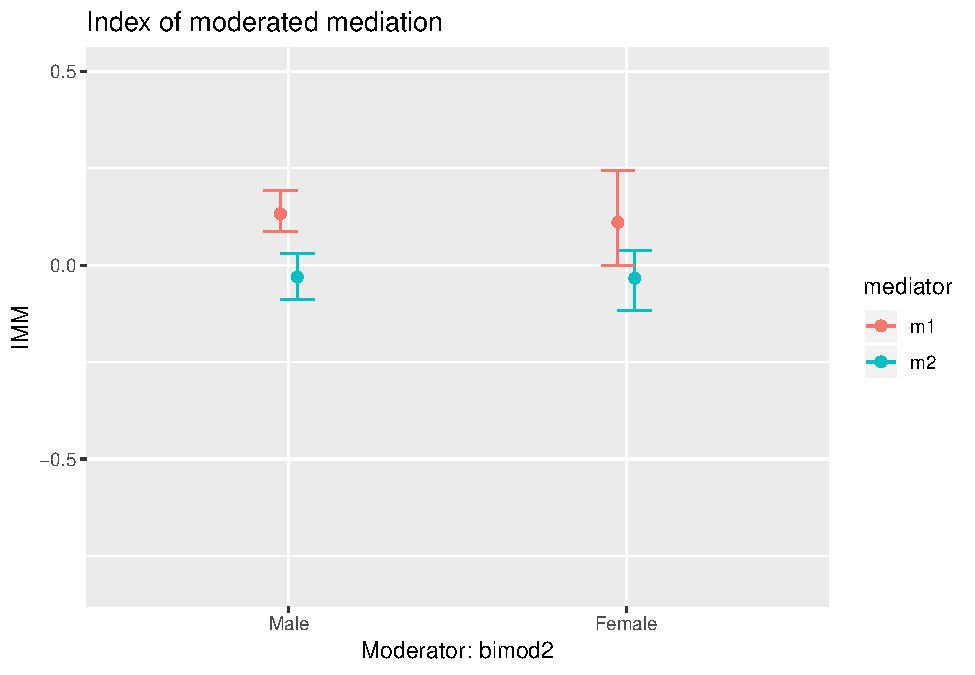
\includegraphics{gemmTutorial_pap__files/figure-latex/model2RIMM-1.pdf}
The IMM for the first mediator (m1) is somewhat larger than for the
second (m2). However, for both mediators the IMM hardly changes between
the two categories of the moderator.

The second plot type is the mediated simple slopes plot. A simple slope
plot shows the indirect effect of the predictor on the dependent
variable through a mediator for usually two characteristic values of the
moderator. Each value of the moderator is represented by a separate
line. Parallel lines indicate absence of moderation and crossing lines
the presence of moderation. The 95\% CI interval around each line is
indicated by a shaded area. For each mediator a separate subplot is
given.

\begin{Shaded}
\begin{Highlighting}[]
\KeywordTok{plotSS}\NormalTok{(result)}
\end{Highlighting}
\end{Shaded}

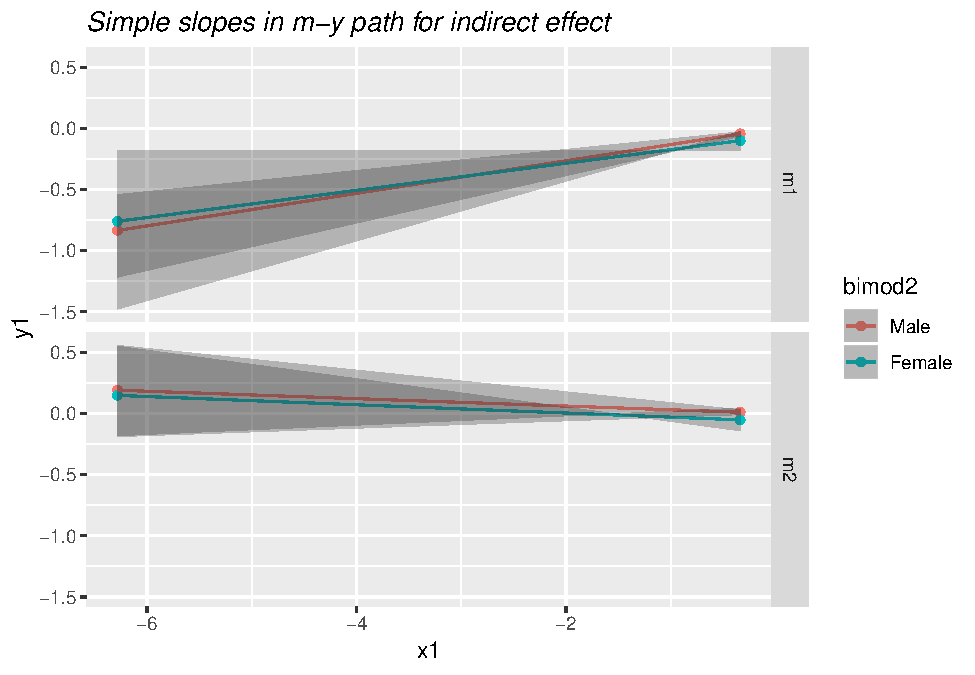
\includegraphics{gemmTutorial_pap__files/figure-latex/model2RSS-1.pdf}
These plots show the effect of the predictor on the dependent variable
through the mediators m1 and m2, respectively. Because the moderator is
a dichotomous variable each plot contains two lines, one for each
category of the moderator.

As a final example we illustrate the use of two numerical moderators.

\begin{Shaded}
\begin{Highlighting}[]
\NormalTok{result <-}\StringTok{ }\KeywordTok{gemm}\NormalTok{(}\DataTypeTok{dat =}\NormalTok{ gemmDat, }
               \DataTypeTok{xvar  =} \StringTok{"x1"}\NormalTok{, }
               \DataTypeTok{mvars =} \KeywordTok{c}\NormalTok{(}\StringTok{"m1"}\NormalTok{,}\StringTok{"m2"}\NormalTok{), }
               \DataTypeTok{yvar  =} \StringTok{"y1"}\NormalTok{,}
               \DataTypeTok{xmmod =} \StringTok{"mod1"}\NormalTok{, }
               \DataTypeTok{mymod =} \StringTok{"mod2"}\NormalTok{,}
               \DataTypeTok{nboot =} \DecValTok{50}\NormalTok{)}

\KeywordTok{plotIMM}\NormalTok{(result)}
\end{Highlighting}
\end{Shaded}

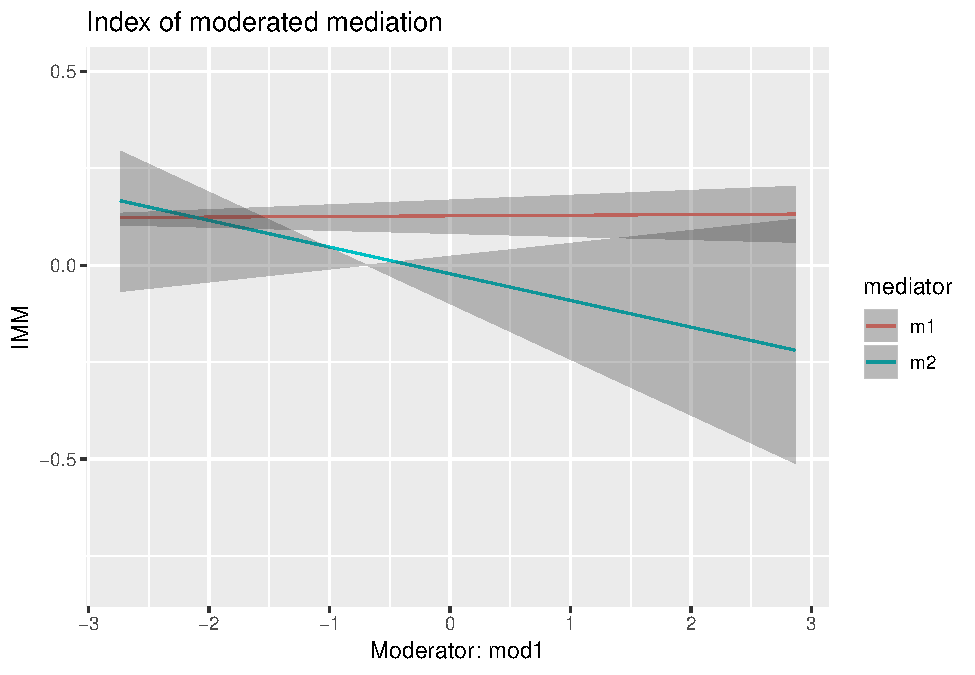
\includegraphics{gemmTutorial_pap__files/figure-latex/model3-1.pdf}
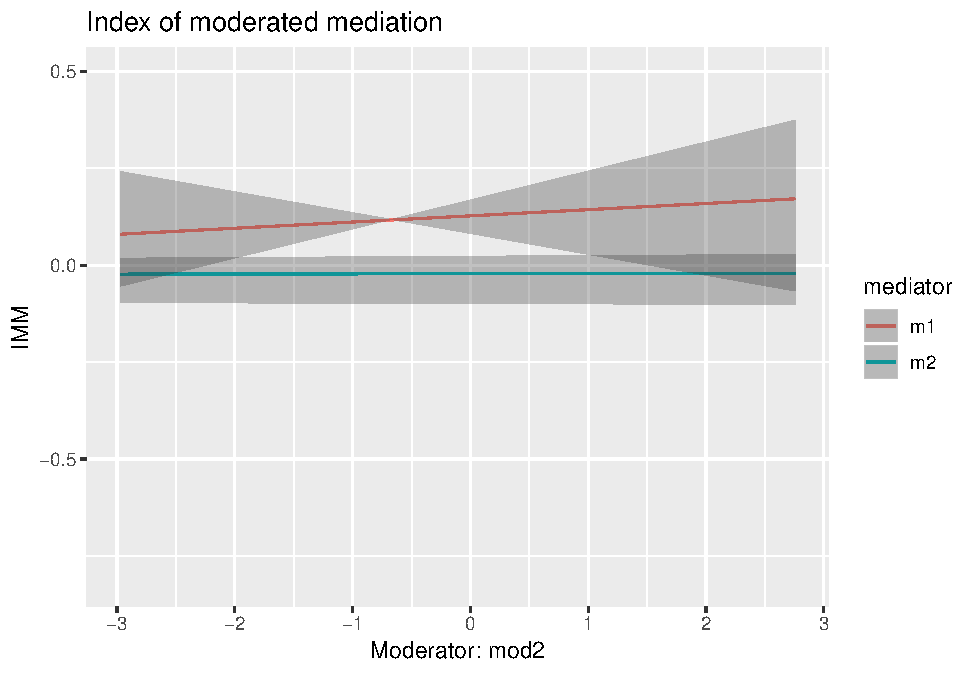
\includegraphics{gemmTutorial_pap__files/figure-latex/model3-2.pdf} The
first plot command provides two plots, for each moderator a separate
plot of the single-path IMM, with in each plot a separate line for each
mediator. In the first plot (for mod1) we see that for the second
mediator the IMM becomes more negative as the value of the moderator
increases. So, the effect of x1 on y1 is more negative for larger values
of mod1.

The second plot command provides a simple slopes plots, one for each
moderator, where each plot is split into subplots for each mediator. The
lines represent the effect evaluated at the 16th and 84th percentile of
the moderator, as recommended by Hayes(2018). Only for mod1 and mediator
m2 there seems moderation, because we can see crossing lines. In the
other three cases the lines run parallel to each other, indicating no
relevant moderation effects.

\begin{Shaded}
\begin{Highlighting}[]
\KeywordTok{plotSS}\NormalTok{(result)}
\end{Highlighting}
\end{Shaded}

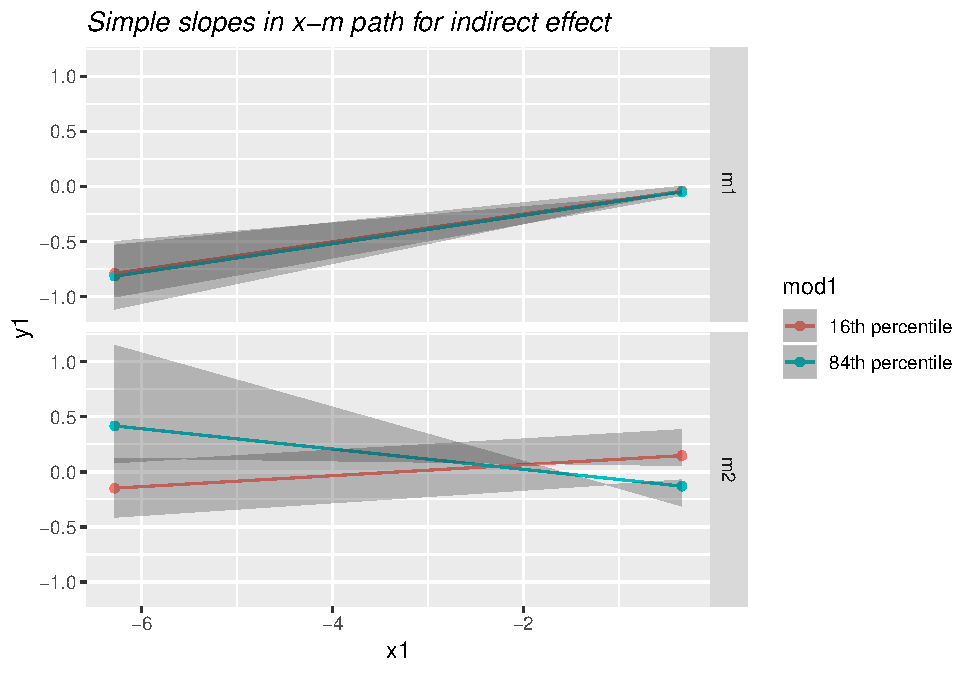
\includegraphics{gemmTutorial_pap__files/figure-latex/model3SS-1.pdf}
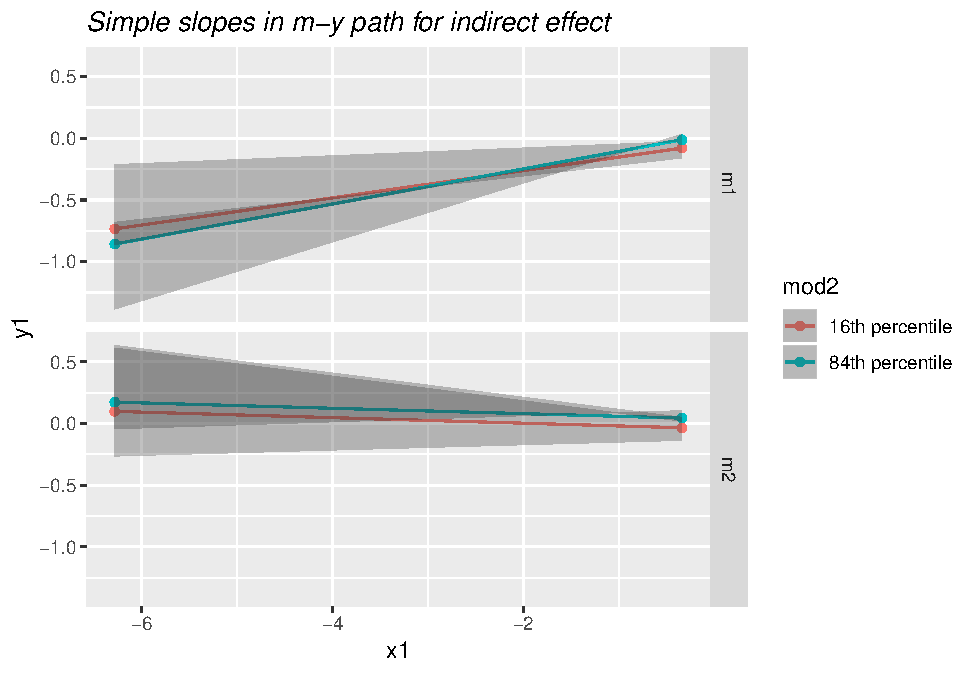
\includegraphics{gemmTutorial_pap__files/figure-latex/model3SS-2.pdf}

The \texttt{plotIMM3d(result)} command provides 3d-plots showing the
double-path IMM for both moderators. Separate plots are given for each
mediator. The message is the same as in the previous plots: only the
moderated mediation effect appears to be present: the indirect effect of
x1 on y through the second mediator is moderated by mod1.

\begin{Shaded}
\begin{Highlighting}[]
\KeywordTok{plotIMM3d}\NormalTok{(result)}
\end{Highlighting}
\end{Shaded}

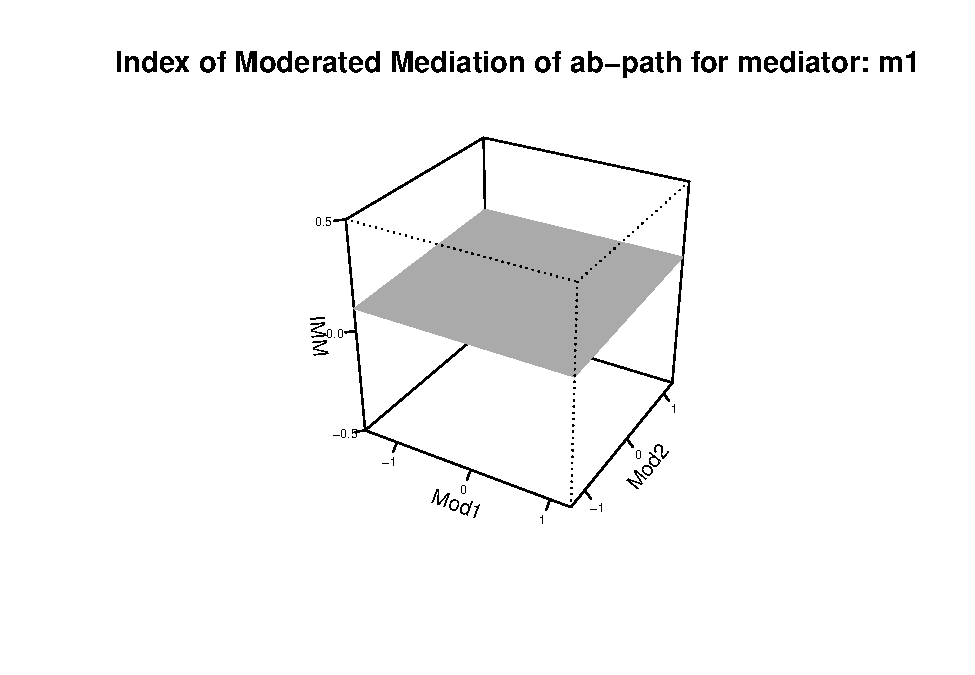
\includegraphics{gemmTutorial_pap__files/figure-latex/model3IMM3d-1.pdf}
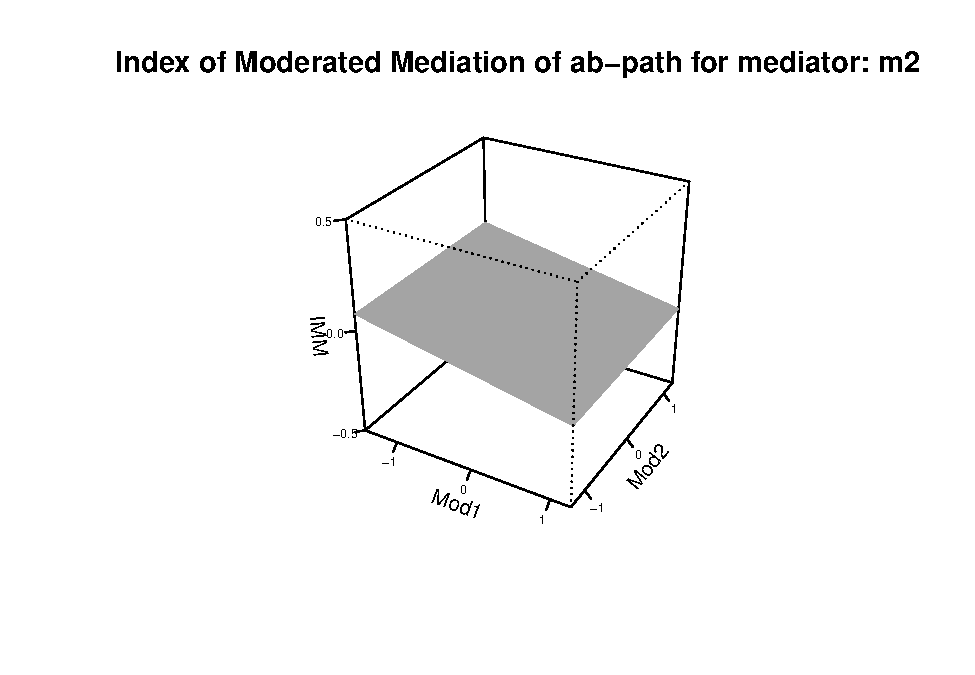
\includegraphics{gemmTutorial_pap__files/figure-latex/model3IMM3d-2.pdf}

\subsection{Additional output}\label{additional-output}

The \texttt{result} object is a list of three elements, which are named
input, intermediate, and results, respectively. Input contains the
original data and all variable names used in the analysis. Intermediate
contains results that have been computed in the functions. For instance
the object \texttt{result\$intermediate\$model} contains the model
specification that was used by lavaan, the object
\texttt{result\$intermediate\$result} contains the output of lavaan. You
can inspect this output by loading the package lavaan and then using
\texttt{summary(result\$intermediate\$result)}. All other lavaan extract
functions can be used on this object. The object
\texttt{result\$intermediate\$parameterEstimates} contains all estimated
parameters from lavaan. For example, when you want to see some important
fit measures obtained in lavaan, you may type:

\begin{Shaded}
\begin{Highlighting}[]
\NormalTok{lavaan}\OperatorTok{::}\KeywordTok{fitmeasures}\NormalTok{(result}\OperatorTok{$}\NormalTok{intermediate}\OperatorTok{$}\NormalTok{result)[}\KeywordTok{c}\NormalTok{(}\StringTok{"cfi"}\NormalTok{,}\StringTok{"tli"}\NormalTok{,}\StringTok{"rmsea"}\NormalTok{,}\StringTok{"chisq"}\NormalTok{, }\StringTok{"df"}\NormalTok{)]}
\end{Highlighting}
\end{Shaded}

\begin{verbatim}
##      cfi      tli    rmsea    chisq       df 
##    0.502   -0.087    0.630 1321.917   11.000
\end{verbatim}

In this way you are able to inspect all other lavaan results.

\subsection{Note}\label{note}

We used R {[}Version 3.5.1; @{]} and the R-packages * base* {[}@
R-base{]}, \emph{gemm} (Version 0.0.1; Verboon, 2018), and \emph{papaja}
(Version 0.1.0.9842; Aust \& Barth, 2018) for all our analyses.

\newpage

\section{References}\label{references}

\begingroup
\setlength{\parindent}{-0.5in} \setlength{\leftskip}{0.5in}

\hypertarget{refs}{}
\hypertarget{ref-R-papaja}{}
Aust, F., \& Barth, M. (2018). \emph{papaja: Create APA manuscripts with
R Markdown}. Retrieved from \url{https://github.com/crsh/papaja}

\hypertarget{ref-Edwards2007}{}
Edwards, J. R., \& Lambert, L. S. (2007). Methods for integrating
moderation and mediation: A general analytical framework using moderated
path analysis. \emph{Psychological Methods}, \emph{12}, 1--22.

\hypertarget{ref-Hayes2015}{}
Hayes, A. F. (2015). An Index and Test of Linear Moderated Mediation.
\emph{Multivariate Behavioral Research}, \emph{50}(1), 1--22.
\url{https://doi.org/10.1080/00273171.2014.962683}

\hypertarget{ref-Hayes2018}{}
Hayes, A. F. (2018). \emph{Introduction to mediation, moderation, and
conditional process analysis}. NY: Guilford Press.

\hypertarget{ref-Preacher2007}{}
Preacher, K. J., Rucker, D. D., \& Hayes, A. F. (2007). Assessing
moderated mediation hypotheses: Theory, methods, and prescriptions.
\emph{Multivariate Behavioral Research}, \emph{42}, 185--227.

\hypertarget{ref-Rosseel2012}{}
Rosseel, Y. (2012). lavaan: An R package for structural equation
modeling. \emph{Journal of Statistical Software}, \emph{48}(2), 1--36.
Retrieved from \url{http://www.jstatsoft.org/v48/i02/}

\hypertarget{ref-R-gemm}{}
Verboon, P. (2018). \emph{Gemm: Moderated mediation with covariates}.

\endgroup


\end{document}
